\begin{statementbox}
\begin{center}\begin{tikzpicture}[font=\small,>=stealth,line join=round]
\draw[gray!40,rounded corners=3pt] (0,0) rectangle (14.2,8.3);\node at (7.1,7.700000000000001) {先看真数，再看底数：都过(1,0)，一升一降};
\begin{scope}[shift={(1.58,3.9499999999999997)},x=1.2cm,y=0.6969696969696969cm]\draw[->,gray] (-0.4,0)--(4.6,0) node[right]{$x$};\draw[->,gray] (0,-3.3)--(0,3.3) node[above]{$y$};\draw[blue!75!black,thick,solid,domain=0.125:4.4,samples=180] plot(\x,{ln(\x)/ln(2)});\draw[orange!85!black,thick,dashed,domain=0.125:4.4,samples=180] plot(\x,{ln(\x)/ln(0.5)});\fill[orange!85!black] (1,0) circle(2.2pt);\fill[orange!85!black] (2,1) circle(2.2pt);\fill[orange!85!black] (2,-1) circle(2.2pt);\fill[orange!85!black] (0.5,-1) circle(2.2pt);\fill[orange!85!black] (0.5,1) circle(2.2pt);\draw[gray!35,densely dotted] (1,0)--(1,-3.3);\node[below=3pt] at (1,-3.3){$1$};\draw[gray!35,densely dotted] (2,0)--(2,-3.3);\node[below=3pt] at (2,-3.3){$2$};\draw[gray!35,densely dotted] (4,0)--(4,-3.3);\node[below=3pt] at (4,-3.3){$4$};\draw[gray,densely dotted] (2,-1)--(2,1);\end{scope}\node[anchor=west,align=left,text width=5.0cm] at (8.4,4.0) {蓝：$\log_2x$，向右上升\\[5pt]橙：$\log_{1/2}x$，向右下降\\[5pt]共同点：$(1,0)$\\[5pt]蓝点：$(2,1),(\frac12,-1)$\\[5pt]橙线上：$(2,-1),(\frac12,1)$\\[5pt]真数$x>0$，函数值可正可负\\[5pt]两条图像关于$x$轴对称};
\node[text width=12.6cm,align=center] at (7.1,.65) {同一个真数对应相反的函数值；与1比较时，以共同点(1,0)为分界。};
\end{tikzpicture}\end{center}

\textbf{核心速记：}$a>0,a\ne1,x>0$；过$(1,0)$；大底升、小底降；真数正，函数值可正可负。


	\end{statementbox}
\clearpage
\begin{statementbox}
\textbf{\textcolor{CStatement}{条件}}
	\begin{description}[style=nextline, leftmargin=2.8em, labelsep=0.5em, itemsep=0.35em]
		\item[\textbf{\textcolor{CStatement}{条件1（底数要求）：}}] $a>0$, $a\neq 1$.
		\item[\textbf{\textcolor{CStatement}{条件2（定义域）：}}] $x>0$.
	\end{description}

	\textbf{\textcolor{CStatement}{结论}}
	\begin{description}[style=nextline, leftmargin=2.8em, labelsep=0.5em, itemsep=0.45em]
		\item[\textbf{\textcolor{CStatement}{结论一（性质总览）：}}]
			\textbf{\textcolor{CStatement}{直观描述：}}
			对数函数定义域为正实数，值域为全体实数，图像过点$(1,0)$。
			\[
				\operatorname{Dom}=(0,+\infty),\quad \operatorname{Ran}=\mathbb{R},\quad f(1)=0.
			\]

		\item[\textbf{\textcolor{CStatement}{结论二（单调与符号）：}}]
			\textbf{\textcolor{CStatement}{直观描述：}}
			底数大于1时函数递增且$x>1$时$y>0$；底数小于1时函数递减且$x>1$时$y<0$。
			\[
				\begin{cases}
					a>1: & f\uparrow,\quad x>1\Rightarrow y>0,\ 0<x<1\Rightarrow y<0,\\[2pt]
					0<a<1: & f\downarrow,\quad x>1\Rightarrow y<0,\ 0<x<1\Rightarrow y>0.
			\end{cases}
			\]
	\end{description}

	
\end{statementbox}
\clearpage
\begin{statementbox}
\textbf{\textcolor{CStatement}{结论三（找图像的三个关键点）：}}
\[
  \log_a1=0,\qquad \log_a a=1,\qquad
  \log_a\frac1a=-1.
\]
因此，对数函数必经$(1,0)$、$(a,1)$和$(1/a,-1)$。想快速画草图，先标这三个点，再判断曲线是向右上升还是下降。

\medskip
\textbf{\textcolor{CStatement}{结论四（注意是哪两条图像对称）：}}
\begin{itemize}[leftmargin=*,itemsep=0.35em,topsep=0.3em]
  \item $y=\log_a x$与$y=\log_{1/a}x$关于\textbf{$x$轴}对称：同一个$x$，两个函数值互为相反数。
  \item $y=a^x$与$y=\log_a x$关于直线\textbf{$y=x$}对称：把点$(u,v)$的两个坐标交换成$(v,u)$。
\end{itemize}

\begin{center}
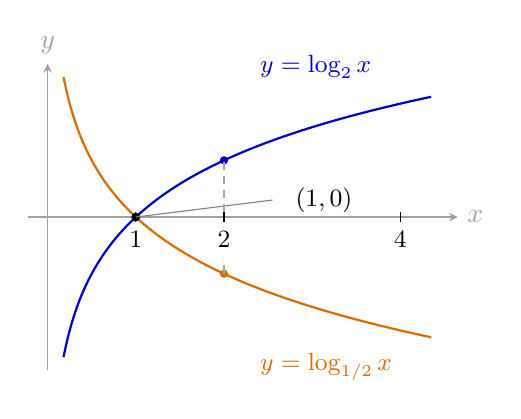
\begin{tikzpicture}[x=1.12cm,y=0.72cm,>=stealth]
  \draw[->,gray!75] (-0.22,0)--(4.65,0) node[right] {$x$};
  \draw[->,gray!75] (0,-2.7)--(0,2.7) node[above] {$y$};
  \foreach \xx in {1,2,4}{\draw (\xx,0.09)--(\xx,-0.09) node[below] {\small $\xx$};}
  \draw[blue!75!black,thick,domain=0.18:4.35,samples=90,smooth] plot (\x,{ln(\x)/ln(2)});
  \draw[orange!85!black,thick,domain=0.18:4.35,samples=90,smooth] plot (\x,{-ln(\x)/ln(2)});
  \fill (1,0) circle (1.6pt) ;\draw[gray] (1,0)--(2.55,.3);\node[anchor=west] at (2.7,.3){\small $(1,0)$};
  \fill[blue!75!black] (2,1) circle (1.5pt);
  \fill[orange!85!black] (2,-1) circle (1.5pt);
  \draw[densely dashed,gray!70] (2,-1)--(2,-.85) (2,.09)--(2,1);
  \node[blue!75!black,anchor=west] at (2.3,2.65) {\small $y=\log_2 x$};
  \node[orange!85!black,anchor=west] at (2.3,-2.65) {\small $y=\log_{1/2}x$};
\end{tikzpicture}
\par\small 图中两条曲线都经过$(1,0)$，并且关于$x$轴上下翻折对应。
\end{center}

\medskip
\textbf{\textcolor{CStatement}{常见变形(底数互倒对称):}}
	\[
		\log_{1/a}x = -\log_a x,
		\qquad
		(a>0,\ a\neq 1).
	\]

\end{statementbox}
